\documentclass{TDP003mall}
\usepackage{float}
\usepackage{graphicx}
\usepackage{pdfpages}
\usepackage{url}




\newcommand{\version}{Version 1.0}
\author{Pia Løtvedt, \url{pialo059@student.liu.se}\\
  Isabella Delgado, \url{isade842@student.liu.se}\\
Sabrina Bjurman, \url{sebbj070@student.liu.se}}

\title{Systemdokumentation}
\date{2017-09-14}
\rhead{Pia Løtvedt\\
  Isabella Delgado\\
  Sabrina Bjurman
}




\begin{document}
\projectpage

\tableofcontents
\pagebreak



\section{Revisionshistorik}
\begin{table}[!h]
\renewcommand{\arraystretch}{1.5}
\begin{tabularx}{\linewidth}{|l|X|l|}
\hline
Ver. & Revisionsbeskrivning & Datum \\
\hline
1.0 & Första version av systemdokumentationen inlämnad &  \\
\hline
\end{tabularx}
\end{table}


\section{Om systemet}
Systemet skapar en portfolio som kan användas av en person för att dokumentera och visa upp de projekt som personen har medverkat i. Portfolion skapas som en webbsida, där det finns möjlighet att läsa om ägaren och ägarens projekt genom att antingen söka bland dem via en avancerad söksida eller en tekniksida där det går att filterera efter vilka tekniker som använts i projektet.

\pagebreak
\section{Översikt över systemets huvudmoduler}


\begin{figure}[h]
  \centering
  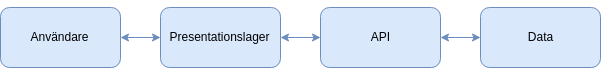
\includegraphics[scale=0.6]{overview}
  \caption{Översikt av systemet}

\end{figure}


Portfolion består av två huvuddelar. Ett datalager som innehåller all information som ska presenteras på webbsidan, samt ett API som hämtar ut denna information i olika format.
Ett presentationslager som sedan använder API:et och genererar portfolions olika sidor med hjälp av den informationen.


\begin{figure}[!]
  \centering
  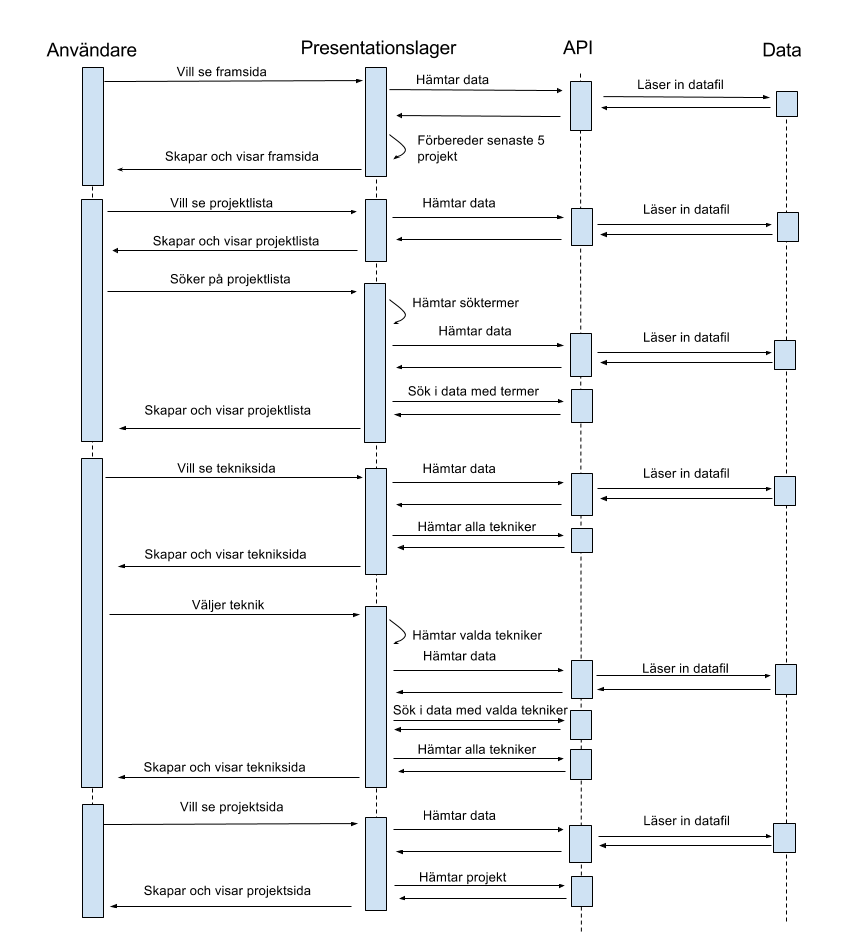
\includegraphics[scale=0.5]{Sekvensdiagram}
  \caption{Sekvensdiagram för systemet}

\end{figure}


\pagebreak
\section{Datalager}

Datalagret består av en fil i JSON-format, som innehåller information om alla projekt som ska presenteras i portfolion, samt ett API, se. \url{http://www.ida.liu.se/~TDP003/current/portfolio-api_python3/}, som kan hämta ut och söka i all denna information på olika sätt.

\subsection{Datafilens struktur}
Data sparas i filen ''ourdata.json'' med JSON-format. Det tar formen av en lista, där varje element är en dictionary som representerar ett projekt. Tabell \ref{table:datafile} visar en lista över vilka nycklar som ingår i varje projekt-dictionary, samt en förklaring till vilka värden dessa nycklar kopplas till.



\begin{table}[!h]
\renewcommand{\arraystretch}{1.5}
\begin{tabularx}{\linewidth}{|l|X|l|l|}
\hline
Nyckel & Beskrivning & Datatyp & Exempel på innehåll \\
\hline
start\_date & Projektets startdatum & sträng & '2009-09-05' \\
\hline
short\_description & Kort beskrivning av projektet & sträng & 'Skapande av portfolio' \\
\hline
course\_name & Om projektet gjordes som en del av en kurs, kursens namn. & sträng & 'Imperativ programmering' \\
\hline
long\_description & Längre beskrivning av projektet & sträng & 'Lång beskrivning' \\
\hline
group\_size & Om projektet gjordes i grupp, gruppens storlek & heltal & 4 \\
\hline
academic\_credits & Om projektet gjordes som en kurs, antal kurspoäng & decimaltal & 7.5  \\
\hline
external\_link & Länk till projektets webbplats & sträng & 'http://portfolio.com' \\
\hline
small\_image & Filnamn på bild från projektet & sträng & 'projekt.png' \\
\hline
techniques\_used & Alla tekniker använda i projektet & Lista av strängar & ['ada', 'python'] \\
\hline
project\_name & Projektets namn & sträng & 'Min portfolio' \\
\hline
course\_id & Om projektet gjordes som en del av en kurs, kursens ID. & sträng & 'TDP003' \\
\hline
end\_date & Projektets slutdatum & sträng & '2010-09-06' \\
\hline
project\_id & Obligatoriskt fält, projektets id i databasen & heltal & 1 \\
\hline
big\_image & Filnamn på bild från projektet & sträng & 'projekt.png' \\
\hline

\end{tabularx}
\caption{Förklaring av nycklar för varje projekt i listan som finns i data.json}
\label{table:datafile}
\end{table}


\subsection{API:ets funktioner}






\pagebreak
\section{Presentationslager}


\begin{figure}[h]
  \centering
  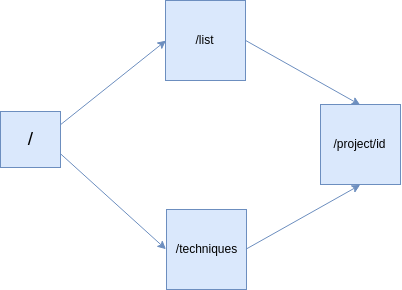
\includegraphics[scale=0.7]{presentationslager}
  \caption{Systemskiss}

\end{figure}


Presentationslagret består bland annat av en huvudfil, myFlaskProject.py som innehåller logiken för de olika sidorna som finns i portfolion. Det är även där som funktionerna i datalagret används. Presentationslagret även av diverse statiska komponenter, såsom bilder, javascript och CSS-filer. Slutligen består presentationslagret av templat för uppbyggnaden av portfolions olika sidor.




\subsection{myFlaskProject.py}

Funktionerna för presentationslagret finns i filen myFlaskProject.py och förklaras mer ingående under rubrik \ref{Bilagor}. Huvudfunktionerna är website\_index, project\_list, project\_techniques och show\_project. Det är dessa funktioner som anropas när en användare försöker navigera till en sida på hemsidan. Utöver huvudfunktionerna så finns det även hjälpfunktioner för att exempelvis hämta data, project eller tekniker, hjälpfunktioner för att hantera GET och POST förfrågningar, och slutligen så finns det även stilfunktioner som används för generera design för vissa element på hemsidan.




\subsection{Statiska komponenter}

Det finns vissa statiska komponenter som behövs för utseendet och funktionaliteten för portfolion. Dessa finns i olika mappar i katalogstrukturen. Mappen med statiska komponenter heter static och innehåller mapparna images, scripts och style.


\begin{figure}[h]
  \centering
  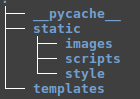
\includegraphics[scale=0.8]{folder_structure}
  \caption{Mappstrukturen för systemet}

\end{figure}


\subsubsection{Bilder}

I mappen images finns det en mapp för varje projekt samt standardbilder som läggs upp på portfoliosidan om ett projekt inte skulle ha någon bild eller ifall bilden skulle ha ett ogiltigt filformat. Bilden för portfolions ägare finns även under denna mapp. För vidare instruktioner hur man lägger in projektbilder och foto på portfolioanvändaren, se README.txt i mappen images.

\subsubsection{Script}

Det finns tre JavaScript-filer som innehåller viss funktionalitet för portfolion, så som kopiering av e-postadress, hover-effekt för projekten och sökningen för portfolion.

\subsubsection{CSS-filer}

Under style-mappen finns det stilmallar för de olika sidorna i portfolion. Bootstrap komponent biblioteket har använts för designen av de olika komponenterna i portfolion.

\subsection{Templat}

Under mappen template finns de html-filer för de olika portfoliosidorna. I dessa filer används Jinja2 för att skriva pythonkod som kan dynamiskt generera de olika html-dokument som hemsidan består av.





\section{Felsökning och felhantering}

Under arbete med portfolion kan fel uppstå på flera olika nivåer. Detta kapitel redogör för vilka metoder och verktyg man kan använda för att undersöka och åtgärda vanliga fel.

Generellt för all felsökning är att det är bra att spara och testa kodens funktion ofta. Om man ändrar en liten del av koden, och det sedan inte fungerar, är det mycket lättare att hitta nyss implementerade fel. Om man däremot har ändrat stora delar av koden utan att kontinuerligt testa, kan felet i princip ligga var som helst, och det kan bli mycket svårare att hitta det.


\subsection{Felsökning med hjälp av Flask}
Under utvecklingen kan fel uppstå i Python-koden eller i Jinja2-templaten som gör att sidan inte kan visas. Förutom syntaxfel i Python-koden, som behandlas nedan, kommer man inte att få ett felmeddelande i terminalfönstret. Istället visas inte sidan när man försöker ladda den. Om man kör appen i vanligt läge kommer sidan att visa ''Internal Server Error''. Under utvecklingsarbetet kan man dock använda debug-läge för att få mer information om felet. Debug-läge aktiveras vid att skicka detta som parameter till run-funktionen i myFlaskProject.py:

\begin{figure}
  \centering
  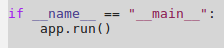
\includegraphics{debugmode}
  \caption{Kod längst ner i myFlaskProject.py för att aktivera debug-läge}
\end{figure}


Fördelen med att använda debugläge är dels att servern automatiskt startas om när man sparar ändringar i en fil, samt att man istället för sidan ''Internal Server Error'' får upp en detaljerad logg över senaste utförda kodrader och en beskrivning av felet.
Debugläget visar information om fel som uppstår både i myFlaskProject.py och i Jinja2-templat.

\textbf{Notera:} Flasks debug-läge ska inte användas på en server som ligger tillgänglig online, då detta utgör en säkerhetsrisk.

\begin{figure}
  \centering
  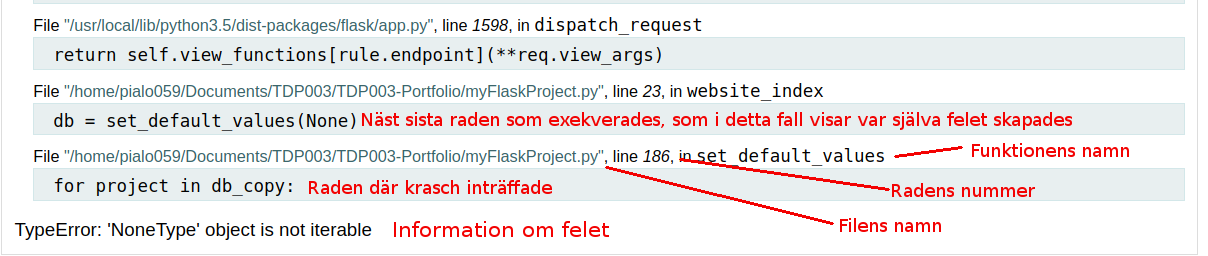
\includegraphics{flaskdebug1}
  \caption{Debuggerns utseende vid fel i myFlaskProject.py. Användbar information är filens namn, exekverade kommandon, radnummer och namn på funktion, samt beskrivning av felet}
\end{figure}

\begin{figure}
  \centering
  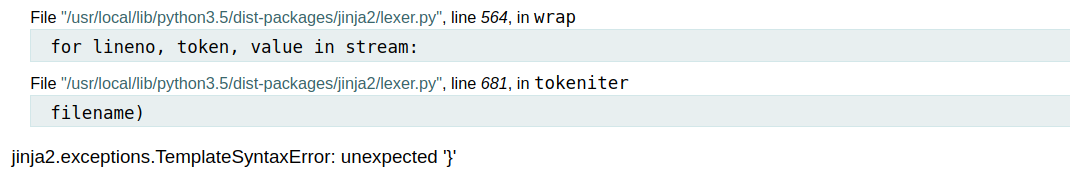
\includegraphics{flaskdebug2}
  \caption{Debuggerns utseende vid fel i ett Jinja2-templat. Användbar information är beskrivning av felet.}
\end{figure}
  

\subsection{Felsökning av Python-kod}
Om utvecklaren inför syntaxfel i Python-koden startar inte servern. Alternativt, om servern har startats i debug-läge, som förklarat ovan, kommer servern att stoppas. Vid omladdning av sidan får man då upp att sidan inte kan nås.
Terminalfönstret innehållar då information om felet, och man kan använda denna information för att hitta var i koden felet har uppstått.

\begin{figure}
  \centering
  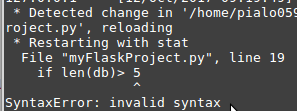
\includegraphics{python_error}
  \caption{Terminalfönstrets utseende vid ett syntaxfel i myFlaskProject.py. Felbeskrivningen innehåller namn på filen, radnummer där felet uppstod, raden som förde till kraschet och en pil som ofta visar exakt var felet ligger i raden}
\end{figure}

\subsection{Felaktigt utseende}
Om sidan laddar, men inte ser ut som förväntat, är det troligt att det finns ett fel i HTML-templatet för sidan. Vid testning i Chrome kan man använda Chromes utvecklarverktyg för att undersöka sidans struktur närmre. Två av dessa verktyg är särskilt till hjälp.

\subsubsection{Sidans källkod}
För att komma åt sidans källkod, högerklicka på sidan och välj ''View page sourse''. Alternativt kan man på en PC klicka Ctrl + U. På sidans källkod kan man hitta den genererade HTML-koden. Detta är till hjälp om man till exempel vill kolla att externa länkar och länkar till filnamn har genererats rätt.

\begin{figure}
  \centering
  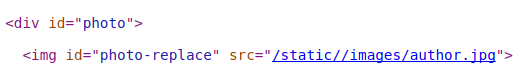
\includegraphics{sourcecode}
  \caption{Fel i genererad bildadress i källkoden}
\end{figure}


\subsubsection{Inspektera HTML-element}
Vid att högerklicka på ett element och välja ''Inspect'' kan man undersöka HTML-kod och CSS för olika sidelement. Detta är ett myket bra verktyg för att felsöka fel i elements utseende, och det kan användas på flera olika sätt. Olika möjligheter i detta verktyg inkluderar:

\begin{itemize}
\item: Se vilka delar av sidan som ingår i olika HTML-element - Underlättar att se fel i placering av taggar för att öppna och stänga element
\item: Se boxmodell av elementet - Underlättar att se fel i storlekar på olika delar (height, width, padding, margin) av elementet.
\item: Se CSS-egenskaper som berör elementet - Underlättar att se om en CSS-egenskap överskrivs av samma CSS-egenskap i en annan klass
\item: Ändra CSS-egenskaper - Möjliggör snabb testning av ändringar av olika egenskaper
\end{itemize}


\begin{figure}
  \centering
  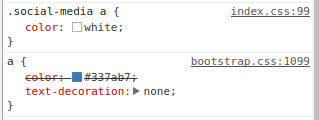
\includegraphics{inspectelement}
  \caption{Undersökning} av CSS-egenskaper i inspektion av element. Här kan man se att a-elementets färg skulle varit hexadecimalt 337ab7 enligt bootstrap.css-filen, men att deta har överskrivits i filen index.css
\end{figure}


\subsection{Felsökning i OpenShift}
Vid uppladdning av portfolion i OpenShift kan olika problem uppstå. OpenShift Client Tools, rhc, inkluderar loggfiler där man kan få information om olika fel som har uppstått. Man kan komma åt en utskrift av de senaste loggar med kommandot \texttt{rhc tail -a appnamn}. Information man kan få från detta verktyg inkluderar problem med att komma åt olika moduler i appen, samt problem med att öppna filer på grund av teckenkodning.





\pagebreak

\includepdf[pages=2,scale=.7,pagecommand=\section{Bilagor}\label{Bilagor}]{api.pdf}
\includepdf[pages=3-4,scale=.7,pagecommand={}]{api.pdf}

\end{document}
